\subsection{Hyper-Parameter Tuning Protocol}\label{sec:tuning-protocol}

In all our experiments, we tune the following optimizer hyper-parameters and otherwise use the PyTorch default values:
\begin{itemize}
\item \textbf{SGD:} learning rate, momentum
\item \textbf{Adam:} learning rate
\item \textbf{Hessian-free:} type of curvature matrix (Hessian or GGN), damping, whether to adapt damping over time (yes or no), maximum number of CG iterations
\item \textbf{LBFGS:} learning rate, history size
\item \textbf{ENGD:} damping, factor of the exponential moving average applied to the Gramian, initialization of the Gramian (zero or identity matrix)
\item \textbf{KFAC:} factor of the exponential moving average applied to the Kronecker factors, damping, momentum, initialization of the Kronecker factors (zero or identity matrix)
\item \textbf{KFAC*:} factor of the exponential moving average applied to the Kronecker factors, damping, initialization of the Kronecker factors (zero or identity matrix)
\end{itemize}

Depending on the optimizer and experiment we use grid, random, or Bayesian search from Weights \& Biases.
Each individual run is allowed to run for a given time budget, and the best run within a search is given by that with lowest final $L_2$ error on a fixed evaluation data set.
All runs are executed on RTX 6000 GPUs with 24\,GiB of RAM to be comparable.
For grid and random searches, we use a round-based approach.
First, we choose a relatively wide search space and limit to approximately 50 runs.
In a second, round, we narrow down the hyper-parameter space based on the first round, then re-run for another approximately 50 runs.
We will release the details of all hyper-parameter search spaces, as well as the hyper-parameters for the best runs in our implementation.

\subsection{2d Poisson Equation}

\paragraph{Setup} We consider a two-dimensional Poisson equation $-\Delta u(x, y) = 2 \pi^2 \sin(\pi x) \sin(\pi y)$ on the unit square $(x,y) \in [0, 1]^2$ with sine product right hand side and zero boundary conditions $u(x, y) = 0$ for $(x,y) \in \partial [0,1]^2$.
We choose a single set of training points with $N_{\Omega} = 900, N_{\partial\Omega} = 120$.
The $L_2$ error is evaluated on a separate set of $\num{9000}$ data points using the known solution $u_{\star}(x, y) = \sin(x) \sin(y)$.
Each run is limited to 1000\,s.
We compare three MLP architectures of increasing size, each of whose linear layers are Tanh-activated except for the final one: a shallow $2\to 64\to 1$ MLP with $D=257$, a five layer $2 \to 64 \to 64 \to 48 \to 48 \to 1$ MLP with $D=\num{9873}$, and a five layer $2 \to 256 \to 256\to 128 \to 128 \to 1$ MLP with $D=\num{116097}$.
For the biggest architecture, full and per-layer ENGD lead to out-of-memory errors.
\Cref{fig:poisson2d-appendix} visualizes the results.

\begin{figure}[!h]
  \centering
  \def\pathToFigs{../kfac_pinns_exp/exp17_groupplot_poisson2d}
  \begin{subfigure}[t]{1.0\linewidth}
    \caption{}\label{subfig:poisson2d-time}
    % trim legend, xlabel and xticklabels
    % [trim={left bottom right top},clip]
    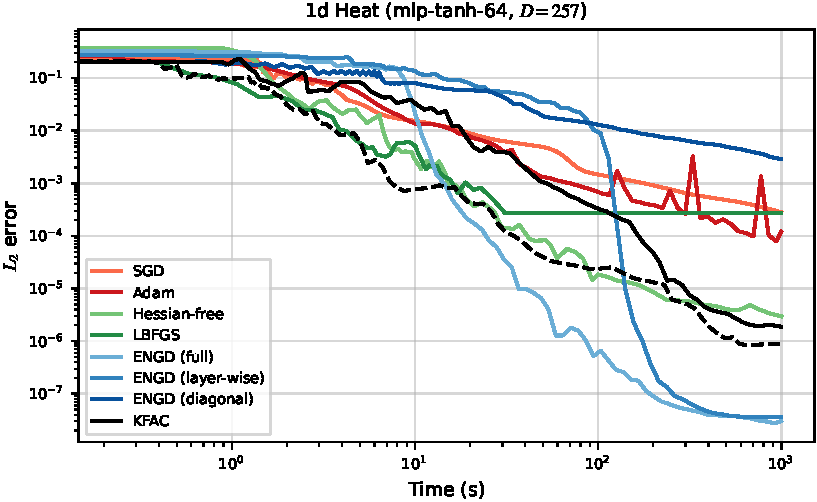
\includegraphics[trim={0 1.3cm 0 0},clip]{\pathToFigs/l2_error_over_time.pdf}
    % trim the legend and titles
    % [trim={left bottom right top},clip]
    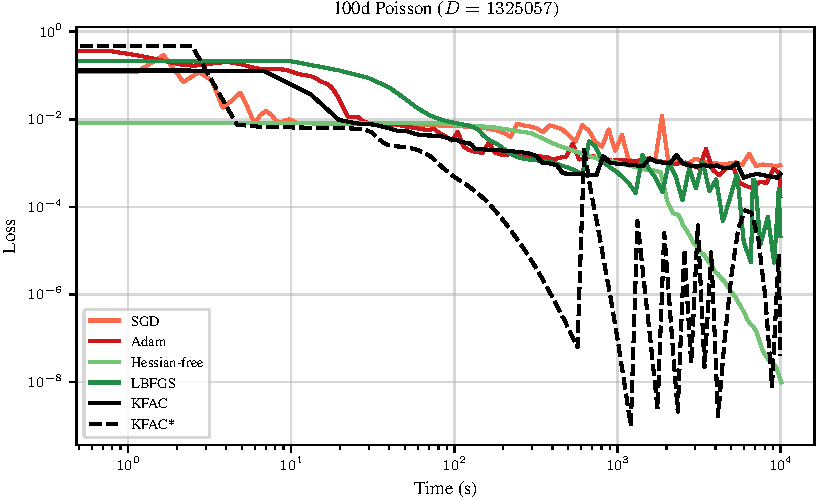
\includegraphics[trim={0 0.5cm 0 0.3cm},clip]{\pathToFigs/loss_over_time.pdf}
  \end{subfigure}
  \begin{subfigure}[t]{1.0\linewidth}
    \caption{}\label{subfig:poisson2d-step}
    % trim the legend, xlabel and xticklabels
    % [trim={left bottom right top},clip]
    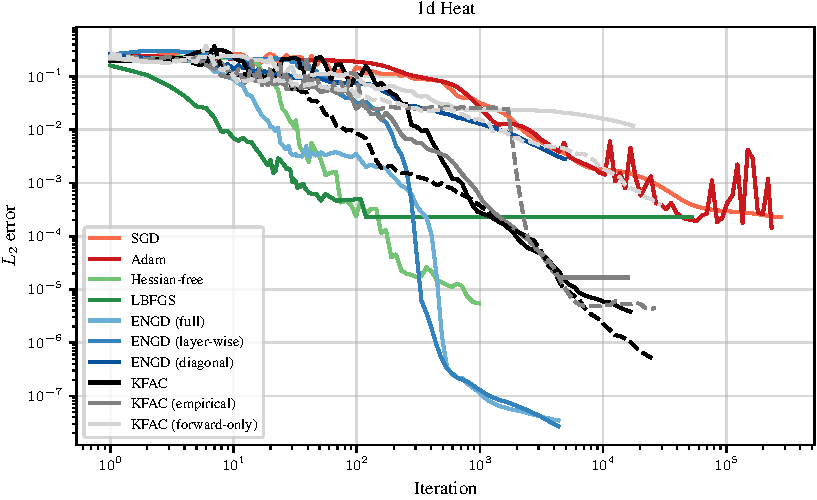
\includegraphics[trim={0 1.3cm 0 0.3cm},clip]{\pathToFigs/l2_error_over_step.pdf}
    % trim the titles
    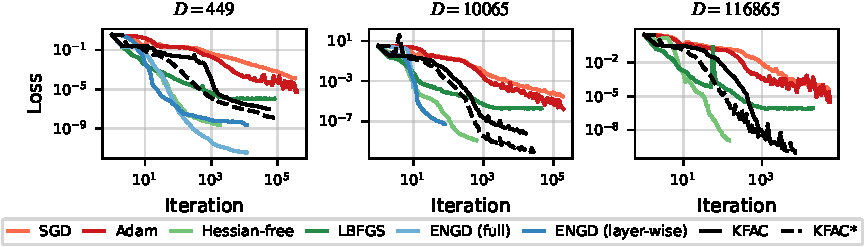
\includegraphics[trim={0 0 0 0.3cm},clip]{\pathToFigs/loss_over_step.pdf}
  \end{subfigure}
  \caption{ Training loss and evaluation $L_2$ error for learning the solution to a 2d Poisson equation over (\subref{subfig:poisson2d-time}) time and (\subref{subfig:poisson2d-step}) steps.
    Columns are different neural networks.}\label{fig:poisson2d-appendix}
\end{figure}

\paragraph{Best run details}
The runs shown in \Cref{fig:poisson2d-appendix} correspond to the following hyper-parameters:
\begin{itemize}
\item $2\to 64\to 1$ MLP with $D=257$
  \begin{itemize}
    \def\pathToRuns{../kfac_pinns_exp/exp09_reproduce_poisson2d/tex}
  \item \textbf{SGD:} learning rate: $\num[scientific-notation=true]{1.007555e-03}$, momentum: $\num[scientific-notation=true]{0.9}$
  \item \textbf{Adam:} learning rate: $\num[scientific-notation=true]{1.369294e-06}$, $N_{\Omega}$: $\num[scientific-notation=false]{203}$, $N_{\partial\Omega}$: $\num[scientific-notation=false]{1494}$, batch sampling frequency: $\num[scientific-notation=false]{9712}$
  \item \textbf{Hessian-free:} curvature matrix: $\text{GGN}$, initial damping: $\num[scientific-notation=true]{1.146081e-02}$, constant damping: $\text{no}$, maximum CG iterations: $\num[scientific-notation=false]{484}$, $N_{\Omega}$: $\num[scientific-notation=false]{2410}$, $N_{\partial\Omega}$: $\num[scientific-notation=false]{2448}$, batch sampling frequency: $\num[scientific-notation=false]{1311}$
  \item \textbf{LBFGS:} learning rate: $\num[scientific-notation=true]{0.2}$, history size: $\num[scientific-notation=false]{225}$
  \item \textbf{ENGD (full):} damping: $\num[scientific-notation=true]{1e-10}$, exponential moving average: $\num[scientific-notation=true]{0.3}$, initialize Gramian to identity: $\text{yes}$
  \item \textbf{ENGD (layer-wise):} damping: $\num[scientific-notation=true]{1e-06}$, exponential moving average: $\num[scientific-notation=true]{0.3}$, initialize Gramian to identity: $\text{no}$
  \item \textbf{KFAC:} damping: $\num[scientific-notation=true]{8.435180e-14}$, momentum: $\num[scientific-notation=true]{9.718645e-01}$, exponential moving average: $\num[scientific-notation=true]{9.800744e-01}$, initialize Kronecker factors to identity: $\text{yes}$, $N_{\Omega}$: $\num[scientific-notation=false]{2525}$, $N_{\partial\Omega}$: $\num[scientific-notation=false]{2663}$, batch sampling frequency: $\num[scientific-notation=false]{7916}$
  \item \textbf{KFAC*:} damping: $\num[scientific-notation=true]{2.965060e-08}$, exponential moving average: $\num[scientific-notation=true]{9.574717e-01}$, initialize Kronecker factors to identity: $\text{yes}$
  \end{itemize}

\item $2 \to 64 \to 64 \to 48 \to 48 \to 1$ MLP with $D=\num{9873}$
  \begin{itemize}
    \def\pathToRuns{../kfac_pinns_exp/exp15_poisson2d_deepwide/tex}
  \item \textbf{SGD:} learning rate: $\num[scientific-notation=true]{1.007555e-03}$, momentum: $\num[scientific-notation=true]{0.9}$
  \item \textbf{Adam:} learning rate: $\num[scientific-notation=true]{1.369294e-06}$, $N_{\Omega}$: $\num[scientific-notation=false]{203}$, $N_{\partial\Omega}$: $\num[scientific-notation=false]{1494}$, batch sampling frequency: $\num[scientific-notation=false]{9712}$
  \item \textbf{Hessian-free:} curvature matrix: $\text{GGN}$, initial damping: $\num[scientific-notation=true]{1.146081e-02}$, constant damping: $\text{no}$, maximum CG iterations: $\num[scientific-notation=false]{484}$, $N_{\Omega}$: $\num[scientific-notation=false]{2410}$, $N_{\partial\Omega}$: $\num[scientific-notation=false]{2448}$, batch sampling frequency: $\num[scientific-notation=false]{1311}$
  \item \textbf{LBFGS:} learning rate: $\num[scientific-notation=true]{0.2}$, history size: $\num[scientific-notation=false]{225}$
  \item \textbf{ENGD (full):} damping: $\num[scientific-notation=true]{1e-10}$, exponential moving average: $\num[scientific-notation=true]{0.3}$, initialize Gramian to identity: $\text{yes}$
  \item \textbf{ENGD (layer-wise):} damping: $\num[scientific-notation=true]{1e-06}$, exponential moving average: $\num[scientific-notation=true]{0.3}$, initialize Gramian to identity: $\text{no}$
  \item \textbf{KFAC:} damping: $\num[scientific-notation=true]{8.435180e-14}$, momentum: $\num[scientific-notation=true]{9.718645e-01}$, exponential moving average: $\num[scientific-notation=true]{9.800744e-01}$, initialize Kronecker factors to identity: $\text{yes}$, $N_{\Omega}$: $\num[scientific-notation=false]{2525}$, $N_{\partial\Omega}$: $\num[scientific-notation=false]{2663}$, batch sampling frequency: $\num[scientific-notation=false]{7916}$
  \item \textbf{KFAC*:} damping: $\num[scientific-notation=true]{2.965060e-08}$, exponential moving average: $\num[scientific-notation=true]{9.574717e-01}$, initialize Kronecker factors to identity: $\text{yes}$
  \end{itemize}

\item $2 \to 256 \to 256\to 128 \to 128 \to 1$ MLP with $D=\num{116097}$
  \begin{itemize}
    \def\pathToRuns{../kfac_pinns_exp/exp20_poisson2d_mlp_tanh_256/tex}
  \item \textbf{SGD:} learning rate: $\num[scientific-notation=true]{1.007555e-03}$, momentum: $\num[scientific-notation=true]{0.9}$
  \item \textbf{Adam:} learning rate: $\num[scientific-notation=true]{1.369294e-06}$, $N_{\Omega}$: $\num[scientific-notation=false]{203}$, $N_{\partial\Omega}$: $\num[scientific-notation=false]{1494}$, batch sampling frequency: $\num[scientific-notation=false]{9712}$
  \item \textbf{Hessian-free:} curvature matrix: $\text{GGN}$, initial damping: $\num[scientific-notation=true]{1.146081e-02}$, constant damping: $\text{no}$, maximum CG iterations: $\num[scientific-notation=false]{484}$, $N_{\Omega}$: $\num[scientific-notation=false]{2410}$, $N_{\partial\Omega}$: $\num[scientific-notation=false]{2448}$, batch sampling frequency: $\num[scientific-notation=false]{1311}$
  \item \textbf{LBFGS:} learning rate: $\num[scientific-notation=true]{0.2}$, history size: $\num[scientific-notation=false]{225}$
  \item \textbf{KFAC:} damping: $\num[scientific-notation=true]{8.435180e-14}$, momentum: $\num[scientific-notation=true]{9.718645e-01}$, exponential moving average: $\num[scientific-notation=true]{9.800744e-01}$, initialize Kronecker factors to identity: $\text{yes}$, $N_{\Omega}$: $\num[scientific-notation=false]{2525}$, $N_{\partial\Omega}$: $\num[scientific-notation=false]{2663}$, batch sampling frequency: $\num[scientific-notation=false]{7916}$
  \item \textbf{KFAC*:} damping: $\num[scientific-notation=true]{2.965060e-08}$, exponential moving average: $\num[scientific-notation=true]{9.574717e-01}$, initialize Kronecker factors to identity: $\text{yes}$
  \end{itemize}
\end{itemize}

\paragraph{Search space details} The runs shown in \Cref{fig:poisson2d-appendix} were determined to be the best via a search with approximately 50 runs on the following search spaces which were obtained by refining an initially wider search ($\mathcal{C}$ denotes a categorical, $\mathcal{U}$ a uniform, and $\mathcal{LU}$ a log-uniform distribution):
\begin{itemize}
\item $2\to 64\to 1$ MLP with $D=257$
  \begin{itemize}
    \def\pathToRuns{../kfac_pinns_exp/exp09_reproduce_poisson2d/tex}
  \item \textbf{SGD:} learning rate: $\mathcal{LU}([\num[scientific-notation=true]{1e-06}; \num[scientific-notation=false]{1}])$, momentum: $\mathcal{U}([\num[scientific-notation=false]{0}; \num[scientific-notation=true]{0.99}])$, $N_{\Omega}$: $\mathcal{C}(\{\num[scientific-notation=false]{100},\num[scientific-notation=false]{101},\text{\dots},\num[scientific-notation=false]{5000}\})$, $N_{\partial\Omega}$: $\mathcal{C}(\{\num[scientific-notation=false]{50},\num[scientific-notation=false]{51},\text{\dots},\num[scientific-notation=false]{2500}\})$, batch sampling frequency: $\mathcal{C}(\{\num[scientific-notation=false]{0},\num[scientific-notation=false]{1},\text{\dots},\num[scientific-notation=false]{1000}\})$
  \item \textbf{Adam:} learning rate: $\mathcal{LU}([\num[scientific-notation=true]{0.0001}; \num[scientific-notation=true]{0.5}])$
  \item \textbf{Hessian-free:} curvature matrix: $\mathcal{U}(\{\text{GGN},\text{Hessian}\})$, initial damping: $\mathcal{LU}([\num[scientific-notation=true]{1e-15}; \num[scientific-notation=false]{1}])$, constant damping: $\mathcal{U}(\{\text{no},\text{yes}\})$, maximum CG iterations: $\mathcal{U}(\{\num[scientific-notation=false]{1},\num[scientific-notation=false]{2},\text{\dots},\num[scientific-notation=false]{500}\})$, $N_{\Omega}$: $\mathcal{U}(\{\num[scientific-notation=false]{100},\num[scientific-notation=false]{101},\text{\dots},\num[scientific-notation=false]{5000}\})$, $N_{\partial\Omega}$: $\mathcal{U}(\{\num[scientific-notation=false]{50},\num[scientific-notation=false]{51},\text{\dots},\num[scientific-notation=false]{2500}\})$, batch sampling frequency: $\mathcal{U}(\{\num[scientific-notation=false]{0},\num[scientific-notation=false]{1},\text{\dots},\num[scientific-notation=false]{5000}\})$
  \item \textbf{LBFGS:} learning rate: $\mathcal{C}(\{\num[scientific-notation=true]{0.5},\num[scientific-notation=true]{0.2},\num[scientific-notation=true]{0.1},\num[scientific-notation=true]{0.05},\num[scientific-notation=true]{0.02},\num[scientific-notation=true]{0.01}\})$, history size: $\mathcal{C}(\{\num[scientific-notation=false]{75},\num[scientific-notation=false]{100},\num[scientific-notation=false]{125},\num[scientific-notation=false]{150},\num[scientific-notation=false]{175},\num[scientific-notation=false]{200},\num[scientific-notation=false]{225},\num[scientific-notation=false]{250}\})$
  \item \textbf{ENGD (full):} damping: $\mathcal{C}(\{\num[scientific-notation=true]{1e-08},\num[scientific-notation=true]{1e-09},\num[scientific-notation=true]{1e-10},\num[scientific-notation=true]{1e-11},\num[scientific-notation=true]{1e-12},\num[scientific-notation=false]{0}\})$, exponential moving average: $\mathcal{C}(\{\num[scientific-notation=false]{0},\num[scientific-notation=true]{0.3},\num[scientific-notation=true]{0.6},\num[scientific-notation=true]{0.9}\})$, initialize Gramian to identity: $\mathcal{C}(\{\text{no},\text{yes}\})$
  \item \textbf{ENGD (layer-wise):} damping: $\mathcal{U}(\{\num[scientific-notation=true]{0.01},\num[scientific-notation=true]{0.001},\num[scientific-notation=true]{0.0001},\num[scientific-notation=true]{1e-05},\num[scientific-notation=true]{1e-06}\})$, exponential moving average: $\mathcal{U}(\{\num[scientific-notation=false]{0},\num[scientific-notation=true]{0.3},\num[scientific-notation=true]{0.6},\num[scientific-notation=true]{0.9},\num[scientific-notation=true]{0.99}\})$, initialize Gramian to identity: $\mathcal{U}(\{\text{no},\text{yes}\})$
  \item \textbf{KFAC:} damping: $\mathcal{LU}([\num[scientific-notation=true]{1e-15}; \num[scientific-notation=true]{0.01}])$, momentum: $\mathcal{U}([\num[scientific-notation=false]{0}; \num[scientific-notation=true]{0.99}])$, exponential moving average: $\mathcal{U}([\num[scientific-notation=false]{0}; \num[scientific-notation=true]{0.99}])$, initialize Kronecker factors to identity: $\mathcal{C}(\{\text{no},\text{yes}\})$
  \item \textbf{KFAC*:} damping: $\mathcal{LU}([\num[scientific-notation=true]{1e-15}; \num[scientific-notation=true]{0.01}])$, exponential moving average: $\mathcal{U}([\num[scientific-notation=false]{0}; \num[scientific-notation=true]{0.99}])$, initialize Kronecker factors to identity: $\mathcal{U}(\{\text{no},\text{yes}\})$, $N_{\Omega}$: $\mathcal{U}(\{\num[scientific-notation=false]{100},\num[scientific-notation=false]{101},\text{\dots},\num[scientific-notation=false]{5000}\})$, $N_{\partial\Omega}$: $\mathcal{U}(\{\num[scientific-notation=false]{50},\num[scientific-notation=false]{51},\text{\dots},\num[scientific-notation=false]{2500}\})$, batch sampling frequency: $\mathcal{U}(\{\num[scientific-notation=false]{0},\num[scientific-notation=false]{1},\text{\dots},\num[scientific-notation=false]{5000}\})$
  \end{itemize}

\item $2 \to 64 \to 64 \to 48 \to 48 \to 1$ MLP with $D=\num{9873}$
  \begin{itemize}
    \def\pathToRuns{../kfac_pinns_exp/exp15_poisson2d_deepwide/tex}
  \item \textbf{SGD:} learning rate: $\mathcal{LU}([\num[scientific-notation=true]{1e-06}; \num[scientific-notation=false]{1}])$, momentum: $\mathcal{U}([\num[scientific-notation=false]{0}; \num[scientific-notation=true]{0.99}])$, $N_{\Omega}$: $\mathcal{C}(\{\num[scientific-notation=false]{100},\num[scientific-notation=false]{101},\text{\dots},\num[scientific-notation=false]{5000}\})$, $N_{\partial\Omega}$: $\mathcal{C}(\{\num[scientific-notation=false]{50},\num[scientific-notation=false]{51},\text{\dots},\num[scientific-notation=false]{2500}\})$, batch sampling frequency: $\mathcal{C}(\{\num[scientific-notation=false]{0},\num[scientific-notation=false]{1},\text{\dots},\num[scientific-notation=false]{1000}\})$
  \item \textbf{Adam:} learning rate: $\mathcal{LU}([\num[scientific-notation=true]{0.0001}; \num[scientific-notation=true]{0.5}])$
  \item \textbf{Hessian-free:} curvature matrix: $\mathcal{U}(\{\text{GGN},\text{Hessian}\})$, initial damping: $\mathcal{LU}([\num[scientific-notation=true]{1e-15}; \num[scientific-notation=false]{1}])$, constant damping: $\mathcal{U}(\{\text{no},\text{yes}\})$, maximum CG iterations: $\mathcal{U}(\{\num[scientific-notation=false]{1},\num[scientific-notation=false]{2},\text{\dots},\num[scientific-notation=false]{500}\})$, $N_{\Omega}$: $\mathcal{U}(\{\num[scientific-notation=false]{100},\num[scientific-notation=false]{101},\text{\dots},\num[scientific-notation=false]{5000}\})$, $N_{\partial\Omega}$: $\mathcal{U}(\{\num[scientific-notation=false]{50},\num[scientific-notation=false]{51},\text{\dots},\num[scientific-notation=false]{2500}\})$, batch sampling frequency: $\mathcal{U}(\{\num[scientific-notation=false]{0},\num[scientific-notation=false]{1},\text{\dots},\num[scientific-notation=false]{5000}\})$
  \item \textbf{LBFGS:} learning rate: $\mathcal{C}(\{\num[scientific-notation=true]{0.5},\num[scientific-notation=true]{0.2},\num[scientific-notation=true]{0.1},\num[scientific-notation=true]{0.05},\num[scientific-notation=true]{0.02},\num[scientific-notation=true]{0.01}\})$, history size: $\mathcal{C}(\{\num[scientific-notation=false]{75},\num[scientific-notation=false]{100},\num[scientific-notation=false]{125},\num[scientific-notation=false]{150},\num[scientific-notation=false]{175},\num[scientific-notation=false]{200},\num[scientific-notation=false]{225},\num[scientific-notation=false]{250}\})$
  \item \textbf{ENGD (full):} damping: $\mathcal{C}(\{\num[scientific-notation=true]{1e-08},\num[scientific-notation=true]{1e-09},\num[scientific-notation=true]{1e-10},\num[scientific-notation=true]{1e-11},\num[scientific-notation=true]{1e-12},\num[scientific-notation=false]{0}\})$, exponential moving average: $\mathcal{C}(\{\num[scientific-notation=false]{0},\num[scientific-notation=true]{0.3},\num[scientific-notation=true]{0.6},\num[scientific-notation=true]{0.9}\})$, initialize Gramian to identity: $\mathcal{C}(\{\text{no},\text{yes}\})$
  \item \textbf{ENGD (layer-wise):} damping: $\mathcal{U}(\{\num[scientific-notation=true]{0.01},\num[scientific-notation=true]{0.001},\num[scientific-notation=true]{0.0001},\num[scientific-notation=true]{1e-05},\num[scientific-notation=true]{1e-06}\})$, exponential moving average: $\mathcal{U}(\{\num[scientific-notation=false]{0},\num[scientific-notation=true]{0.3},\num[scientific-notation=true]{0.6},\num[scientific-notation=true]{0.9},\num[scientific-notation=true]{0.99}\})$, initialize Gramian to identity: $\mathcal{U}(\{\text{no},\text{yes}\})$
  \item \textbf{KFAC:} damping: $\mathcal{LU}([\num[scientific-notation=true]{1e-15}; \num[scientific-notation=true]{0.01}])$, momentum: $\mathcal{U}([\num[scientific-notation=false]{0}; \num[scientific-notation=true]{0.99}])$, exponential moving average: $\mathcal{U}([\num[scientific-notation=false]{0}; \num[scientific-notation=true]{0.99}])$, initialize Kronecker factors to identity: $\mathcal{C}(\{\text{no},\text{yes}\})$
  \item \textbf{KFAC*:} damping: $\mathcal{LU}([\num[scientific-notation=true]{1e-15}; \num[scientific-notation=true]{0.01}])$, exponential moving average: $\mathcal{U}([\num[scientific-notation=false]{0}; \num[scientific-notation=true]{0.99}])$, initialize Kronecker factors to identity: $\mathcal{U}(\{\text{no},\text{yes}\})$, $N_{\Omega}$: $\mathcal{U}(\{\num[scientific-notation=false]{100},\num[scientific-notation=false]{101},\text{\dots},\num[scientific-notation=false]{5000}\})$, $N_{\partial\Omega}$: $\mathcal{U}(\{\num[scientific-notation=false]{50},\num[scientific-notation=false]{51},\text{\dots},\num[scientific-notation=false]{2500}\})$, batch sampling frequency: $\mathcal{U}(\{\num[scientific-notation=false]{0},\num[scientific-notation=false]{1},\text{\dots},\num[scientific-notation=false]{5000}\})$
  \end{itemize}

\item $2 \to 256 \to 256\to 128 \to 128 \to 1$ MLP with $D=\num{116097}$
  \begin{itemize}
    \def\pathToRuns{../kfac_pinns_exp/exp20_poisson2d_mlp_tanh_256/tex}
  \item \textbf{SGD:} learning rate: $\mathcal{LU}([\num[scientific-notation=true]{1e-06}; \num[scientific-notation=false]{1}])$, momentum: $\mathcal{U}([\num[scientific-notation=false]{0}; \num[scientific-notation=true]{0.99}])$, $N_{\Omega}$: $\mathcal{C}(\{\num[scientific-notation=false]{100},\num[scientific-notation=false]{101},\text{\dots},\num[scientific-notation=false]{5000}\})$, $N_{\partial\Omega}$: $\mathcal{C}(\{\num[scientific-notation=false]{50},\num[scientific-notation=false]{51},\text{\dots},\num[scientific-notation=false]{2500}\})$, batch sampling frequency: $\mathcal{C}(\{\num[scientific-notation=false]{0},\num[scientific-notation=false]{1},\text{\dots},\num[scientific-notation=false]{1000}\})$
  \item \textbf{Adam:} learning rate: $\mathcal{LU}([\num[scientific-notation=true]{0.0001}; \num[scientific-notation=true]{0.5}])$
  \item \textbf{Hessian-free:} curvature matrix: $\mathcal{U}(\{\text{GGN},\text{Hessian}\})$, initial damping: $\mathcal{LU}([\num[scientific-notation=true]{1e-15}; \num[scientific-notation=false]{1}])$, constant damping: $\mathcal{U}(\{\text{no},\text{yes}\})$, maximum CG iterations: $\mathcal{U}(\{\num[scientific-notation=false]{1},\num[scientific-notation=false]{2},\text{\dots},\num[scientific-notation=false]{500}\})$, $N_{\Omega}$: $\mathcal{U}(\{\num[scientific-notation=false]{100},\num[scientific-notation=false]{101},\text{\dots},\num[scientific-notation=false]{5000}\})$, $N_{\partial\Omega}$: $\mathcal{U}(\{\num[scientific-notation=false]{50},\num[scientific-notation=false]{51},\text{\dots},\num[scientific-notation=false]{2500}\})$, batch sampling frequency: $\mathcal{U}(\{\num[scientific-notation=false]{0},\num[scientific-notation=false]{1},\text{\dots},\num[scientific-notation=false]{5000}\})$
  \item \textbf{LBFGS:} learning rate: $\mathcal{C}(\{\num[scientific-notation=true]{0.5},\num[scientific-notation=true]{0.2},\num[scientific-notation=true]{0.1},\num[scientific-notation=true]{0.05},\num[scientific-notation=true]{0.02},\num[scientific-notation=true]{0.01}\})$, history size: $\mathcal{C}(\{\num[scientific-notation=false]{75},\num[scientific-notation=false]{100},\num[scientific-notation=false]{125},\num[scientific-notation=false]{150},\num[scientific-notation=false]{175},\num[scientific-notation=false]{200},\num[scientific-notation=false]{225},\num[scientific-notation=false]{250}\})$
  \item \textbf{KFAC:} damping: $\mathcal{LU}([\num[scientific-notation=true]{1e-15}; \num[scientific-notation=true]{0.01}])$, momentum: $\mathcal{U}([\num[scientific-notation=false]{0}; \num[scientific-notation=true]{0.99}])$, exponential moving average: $\mathcal{U}([\num[scientific-notation=false]{0}; \num[scientific-notation=true]{0.99}])$, initialize Kronecker factors to identity: $\mathcal{C}(\{\text{no},\text{yes}\})$
  \item \textbf{KFAC*:} damping: $\mathcal{LU}([\num[scientific-notation=true]{1e-15}; \num[scientific-notation=true]{0.01}])$, exponential moving average: $\mathcal{U}([\num[scientific-notation=false]{0}; \num[scientific-notation=true]{0.99}])$, initialize Kronecker factors to identity: $\mathcal{U}(\{\text{no},\text{yes}\})$, $N_{\Omega}$: $\mathcal{U}(\{\num[scientific-notation=false]{100},\num[scientific-notation=false]{101},\text{\dots},\num[scientific-notation=false]{5000}\})$, $N_{\partial\Omega}$: $\mathcal{U}(\{\num[scientific-notation=false]{50},\num[scientific-notation=false]{51},\text{\dots},\num[scientific-notation=false]{2500}\})$, batch sampling frequency: $\mathcal{U}(\{\num[scientific-notation=false]{0},\num[scientific-notation=false]{1},\text{\dots},\num[scientific-notation=false]{5000}\})$
  \end{itemize}
\end{itemize}

\subsection{5d Poisson Equation}

\paragraph{Setup} We consider a five-dimensional Poisson equation $-\Delta u(\vx) = \pi^2 \sum_{i=1}^5 \cos(\pi \evx_i)$ on the five-dimensional unit square $\vx \in [0, 1]^5$ with cosine sum right hand side and boundary conditions $u(\vx) = \sum_{i=1}^5 \cos(\pi \evx_i)$ for $\vx \in \partial [0,1]^5$.
We sample training batches of size $N_{\Omega} = \num{3000}, N_{\partial\Omega} = 500$ and evaluate the $L_2$ error on a separate set of $\num{30000}$ data points using the known solution $u_{\star}(\vx) = \sum_{i=1}^5 \cos(\pi \evx_i)$.
All optimizers except for KFAC sample a new training batch each iteration.
KFAC only re-samples every 100 iterations because we noticed it works significantly better with multiple iterations on a fixed batch.
To make sure that this does not lead to an unfair advantage of KFAC, we conduct an additional experiment where we also tune the batch sampling frequency, as well as other hyper-parameters; see \Cref{sec:high-dimensional-poissons-app}.
The results presented in this section are consistent with this additional experiment.
Each run is limited to 3000\,s.
We compare three MLP architectures of increasing size, each of whose linear layers are Tanh-activated except for the final one: a shallow $5\to 64\to 1$ MLP with $D=449$, a five layer $5 \to 64 \to 64 \to 48 \to 48 \to 1$ MLP with $D=\num{10065}$, and a five layer $5 \to 256 \to 256\to 128 \to 128 \to 1$ MLP with $D=\num{116864}$.
For the biggest architecture, full and layer-wise ENGD lead to out-of-memory errors.
\Cref{fig:poisson5d-appendix} visualizes the results.

\begin{figure}[!h]
  \centering
  \def\pathToFigs{../kfac_pinns_exp/exp18_groupplot_poisson5d}
  \begin{subfigure}[t]{1.0\linewidth}
    \caption{}\label{subfig:poisson5d-time}
    % trim legend, xlabel and xticklabels
    % [trim={left bottom right top},clip]
    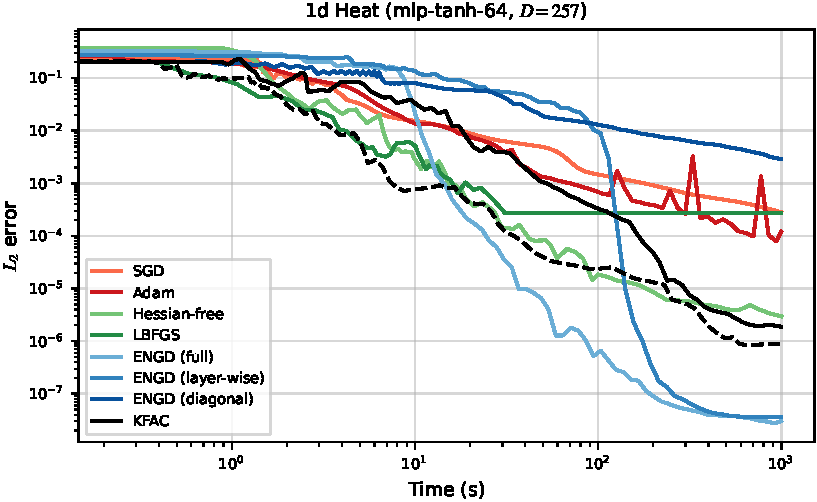
\includegraphics[trim={0 1.3cm 0 0},clip]{\pathToFigs/l2_error_over_time.pdf}
    % trim the legend and titles
    % [trim={left bottom right top},clip]
    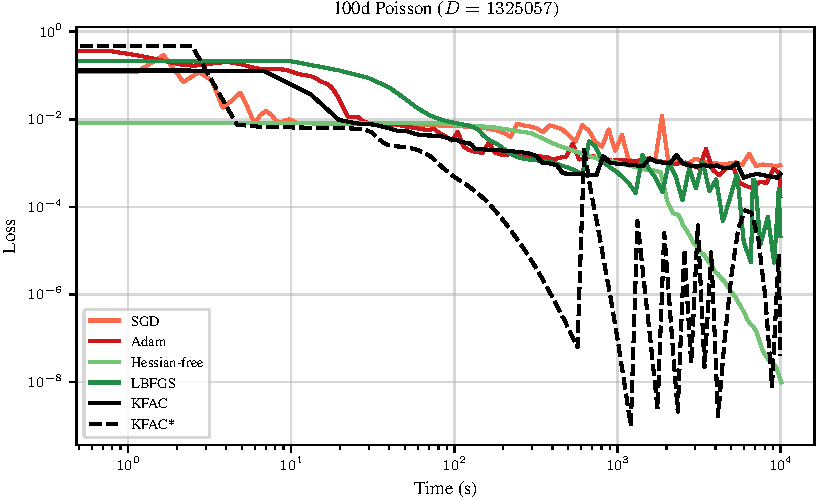
\includegraphics[trim={0 0.5cm 0 0.3cm},clip]{\pathToFigs/loss_over_time.pdf}
  \end{subfigure}
  \begin{subfigure}[t]{1.0\linewidth}
    \caption{}\label{subfig:poisson5d-step}
    % trim the legend, xlabel and xticklabels
    % [trim={left bottom right top},clip]
    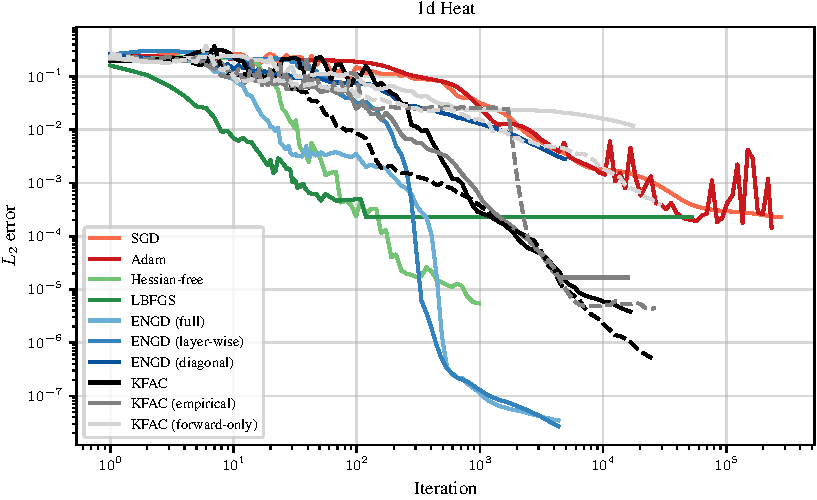
\includegraphics[trim={0 1.3cm 0 0.3cm},clip]{\pathToFigs/l2_error_over_step.pdf}
    % trim the titles
    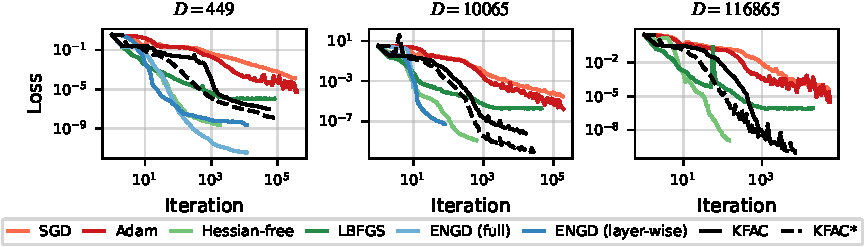
\includegraphics[trim={0 0 0 0.3cm},clip]{\pathToFigs/loss_over_step.pdf}
  \end{subfigure}
  \caption{Training loss and evaluation $L_2$ error for learning the solution to a 5d Poisson equation over (\subref{subfig:poisson5d-time}) time and (\subref{subfig:poisson5d-step}) steps.
    Columns are different neural networks.}\label{fig:poisson5d-appendix}
\end{figure}

\paragraph{Best run details}
The runs shown in \Cref{fig:poisson5d-appendix} correspond to the following hyper-parameters:
\begin{itemize}
\item $5\to 64\to 1$ MLP with $D=449$
  \begin{itemize}
    \def\pathToRuns{../kfac_pinns_exp/exp10_reproduce_poisson5d/tex}
  \item \textbf{SGD:} learning rate: $\num[scientific-notation=true]{1.007555e-03}$, momentum: $\num[scientific-notation=true]{0.9}$
  \item \textbf{Adam:} learning rate: $\num[scientific-notation=true]{1.369294e-06}$, $N_{\Omega}$: $\num[scientific-notation=false]{203}$, $N_{\partial\Omega}$: $\num[scientific-notation=false]{1494}$, batch sampling frequency: $\num[scientific-notation=false]{9712}$
  \item \textbf{Hessian-free:} curvature matrix: $\text{GGN}$, initial damping: $\num[scientific-notation=true]{1.146081e-02}$, constant damping: $\text{no}$, maximum CG iterations: $\num[scientific-notation=false]{484}$, $N_{\Omega}$: $\num[scientific-notation=false]{2410}$, $N_{\partial\Omega}$: $\num[scientific-notation=false]{2448}$, batch sampling frequency: $\num[scientific-notation=false]{1311}$
  \item \textbf{LBFGS:} learning rate: $\num[scientific-notation=true]{0.2}$, history size: $\num[scientific-notation=false]{225}$
  \item \textbf{ENGD (full):} damping: $\num[scientific-notation=true]{1e-10}$, exponential moving average: $\num[scientific-notation=true]{0.3}$, initialize Gramian to identity: $\text{yes}$
  \item \textbf{ENGD (layer-wise):} damping: $\num[scientific-notation=true]{1e-06}$, exponential moving average: $\num[scientific-notation=true]{0.3}$, initialize Gramian to identity: $\text{no}$
  \item \textbf{KFAC:} damping: $\num[scientific-notation=true]{8.435180e-14}$, momentum: $\num[scientific-notation=true]{9.718645e-01}$, exponential moving average: $\num[scientific-notation=true]{9.800744e-01}$, initialize Kronecker factors to identity: $\text{yes}$, $N_{\Omega}$: $\num[scientific-notation=false]{2525}$, $N_{\partial\Omega}$: $\num[scientific-notation=false]{2663}$, batch sampling frequency: $\num[scientific-notation=false]{7916}$
  \item \textbf{KFAC*:} damping: $\num[scientific-notation=true]{2.965060e-08}$, exponential moving average: $\num[scientific-notation=true]{9.574717e-01}$, initialize Kronecker factors to identity: $\text{yes}$
  \end{itemize}

\item $5 \to 64 \to 64 \to 48 \to 48 \to 1$ MLP with $D=\num{10065}$
  \begin{itemize}
    \def\pathToRuns{../kfac_pinns_exp/exp16_poisson5d_deepwide/tex}
  \item \textbf{SGD:} learning rate: $\num[scientific-notation=true]{1.007555e-03}$, momentum: $\num[scientific-notation=true]{0.9}$
  \item \textbf{Adam:} learning rate: $\num[scientific-notation=true]{1.369294e-06}$, $N_{\Omega}$: $\num[scientific-notation=false]{203}$, $N_{\partial\Omega}$: $\num[scientific-notation=false]{1494}$, batch sampling frequency: $\num[scientific-notation=false]{9712}$
  \item \textbf{Hessian-free:} curvature matrix: $\text{GGN}$, initial damping: $\num[scientific-notation=true]{1.146081e-02}$, constant damping: $\text{no}$, maximum CG iterations: $\num[scientific-notation=false]{484}$, $N_{\Omega}$: $\num[scientific-notation=false]{2410}$, $N_{\partial\Omega}$: $\num[scientific-notation=false]{2448}$, batch sampling frequency: $\num[scientific-notation=false]{1311}$
  \item \textbf{LBFGS:} learning rate: $\num[scientific-notation=true]{0.2}$, history size: $\num[scientific-notation=false]{225}$
  \item \textbf{ENGD (full):} damping: $\num[scientific-notation=true]{1e-10}$, exponential moving average: $\num[scientific-notation=true]{0.3}$, initialize Gramian to identity: $\text{yes}$
  \item \textbf{ENGD (layer-wise):} damping: $\num[scientific-notation=true]{1e-06}$, exponential moving average: $\num[scientific-notation=true]{0.3}$, initialize Gramian to identity: $\text{no}$
  \item \textbf{KFAC:} damping: $\num[scientific-notation=true]{8.435180e-14}$, momentum: $\num[scientific-notation=true]{9.718645e-01}$, exponential moving average: $\num[scientific-notation=true]{9.800744e-01}$, initialize Kronecker factors to identity: $\text{yes}$, $N_{\Omega}$: $\num[scientific-notation=false]{2525}$, $N_{\partial\Omega}$: $\num[scientific-notation=false]{2663}$, batch sampling frequency: $\num[scientific-notation=false]{7916}$
  \item \textbf{KFAC*:} damping: $\num[scientific-notation=true]{2.965060e-08}$, exponential moving average: $\num[scientific-notation=true]{9.574717e-01}$, initialize Kronecker factors to identity: $\text{yes}$
  \end{itemize}

\item $5 \to 256 \to 256\to 128 \to 128 \to 1$ MLP with $D=\num{116865}$
  \begin{itemize}
    \def\pathToRuns{../kfac_pinns_exp/exp19_poisson5d_mlp_tanh_256/tex}
  \item \textbf{SGD:} learning rate: $\num[scientific-notation=true]{1.007555e-03}$, momentum: $\num[scientific-notation=true]{0.9}$
  \item \textbf{Adam:} learning rate: $\num[scientific-notation=true]{1.369294e-06}$, $N_{\Omega}$: $\num[scientific-notation=false]{203}$, $N_{\partial\Omega}$: $\num[scientific-notation=false]{1494}$, batch sampling frequency: $\num[scientific-notation=false]{9712}$
  \item \textbf{Hessian-free:} curvature matrix: $\text{GGN}$, initial damping: $\num[scientific-notation=true]{1.146081e-02}$, constant damping: $\text{no}$, maximum CG iterations: $\num[scientific-notation=false]{484}$, $N_{\Omega}$: $\num[scientific-notation=false]{2410}$, $N_{\partial\Omega}$: $\num[scientific-notation=false]{2448}$, batch sampling frequency: $\num[scientific-notation=false]{1311}$
  \item \textbf{LBFGS:} learning rate: $\num[scientific-notation=true]{0.2}$, history size: $\num[scientific-notation=false]{225}$
  \item \textbf{KFAC:} damping: $\num[scientific-notation=true]{8.435180e-14}$, momentum: $\num[scientific-notation=true]{9.718645e-01}$, exponential moving average: $\num[scientific-notation=true]{9.800744e-01}$, initialize Kronecker factors to identity: $\text{yes}$, $N_{\Omega}$: $\num[scientific-notation=false]{2525}$, $N_{\partial\Omega}$: $\num[scientific-notation=false]{2663}$, batch sampling frequency: $\num[scientific-notation=false]{7916}$
  \item \textbf{KFAC*:} damping: $\num[scientific-notation=true]{2.965060e-08}$, exponential moving average: $\num[scientific-notation=true]{9.574717e-01}$, initialize Kronecker factors to identity: $\text{yes}$
  \end{itemize}
\end{itemize}

\paragraph{Search space details} The runs shown in \Cref{fig:poisson5d-appendix} were determined to be the best via a search with approximately 50 runs on the following search spaces which were obtained by refining an initially wider search ($\mathcal{C}$ denotes a categorical, $\mathcal{U}$ a uniform, and $\mathcal{LU}$ a log-uniform distribution):
\begin{itemize}
\item $5\to 64\to 1$ MLP with $D=449$
  \begin{itemize}
    \def\pathToRuns{../kfac_pinns_exp/exp10_reproduce_poisson5d/tex}
  \item \textbf{SGD:} learning rate: $\mathcal{LU}([\num[scientific-notation=true]{1e-06}; \num[scientific-notation=false]{1}])$, momentum: $\mathcal{U}([\num[scientific-notation=false]{0}; \num[scientific-notation=true]{0.99}])$, $N_{\Omega}$: $\mathcal{C}(\{\num[scientific-notation=false]{100},\num[scientific-notation=false]{101},\text{\dots},\num[scientific-notation=false]{5000}\})$, $N_{\partial\Omega}$: $\mathcal{C}(\{\num[scientific-notation=false]{50},\num[scientific-notation=false]{51},\text{\dots},\num[scientific-notation=false]{2500}\})$, batch sampling frequency: $\mathcal{C}(\{\num[scientific-notation=false]{0},\num[scientific-notation=false]{1},\text{\dots},\num[scientific-notation=false]{1000}\})$
  \item \textbf{Adam:} learning rate: $\mathcal{LU}([\num[scientific-notation=true]{0.0001}; \num[scientific-notation=true]{0.5}])$
  \item \textbf{Hessian-free:} curvature matrix: $\mathcal{U}(\{\text{GGN},\text{Hessian}\})$, initial damping: $\mathcal{LU}([\num[scientific-notation=true]{1e-15}; \num[scientific-notation=false]{1}])$, constant damping: $\mathcal{U}(\{\text{no},\text{yes}\})$, maximum CG iterations: $\mathcal{U}(\{\num[scientific-notation=false]{1},\num[scientific-notation=false]{2},\text{\dots},\num[scientific-notation=false]{500}\})$, $N_{\Omega}$: $\mathcal{U}(\{\num[scientific-notation=false]{100},\num[scientific-notation=false]{101},\text{\dots},\num[scientific-notation=false]{5000}\})$, $N_{\partial\Omega}$: $\mathcal{U}(\{\num[scientific-notation=false]{50},\num[scientific-notation=false]{51},\text{\dots},\num[scientific-notation=false]{2500}\})$, batch sampling frequency: $\mathcal{U}(\{\num[scientific-notation=false]{0},\num[scientific-notation=false]{1},\text{\dots},\num[scientific-notation=false]{5000}\})$
  \item \textbf{LBFGS:} learning rate: $\mathcal{C}(\{\num[scientific-notation=true]{0.5},\num[scientific-notation=true]{0.2},\num[scientific-notation=true]{0.1},\num[scientific-notation=true]{0.05},\num[scientific-notation=true]{0.02},\num[scientific-notation=true]{0.01}\})$, history size: $\mathcal{C}(\{\num[scientific-notation=false]{75},\num[scientific-notation=false]{100},\num[scientific-notation=false]{125},\num[scientific-notation=false]{150},\num[scientific-notation=false]{175},\num[scientific-notation=false]{200},\num[scientific-notation=false]{225},\num[scientific-notation=false]{250}\})$
  \item \textbf{ENGD (full):} damping: $\mathcal{C}(\{\num[scientific-notation=true]{1e-08},\num[scientific-notation=true]{1e-09},\num[scientific-notation=true]{1e-10},\num[scientific-notation=true]{1e-11},\num[scientific-notation=true]{1e-12},\num[scientific-notation=false]{0}\})$, exponential moving average: $\mathcal{C}(\{\num[scientific-notation=false]{0},\num[scientific-notation=true]{0.3},\num[scientific-notation=true]{0.6},\num[scientific-notation=true]{0.9}\})$, initialize Gramian to identity: $\mathcal{C}(\{\text{no},\text{yes}\})$
  \item \textbf{ENGD (layer-wise):} damping: $\mathcal{U}(\{\num[scientific-notation=true]{0.01},\num[scientific-notation=true]{0.001},\num[scientific-notation=true]{0.0001},\num[scientific-notation=true]{1e-05},\num[scientific-notation=true]{1e-06}\})$, exponential moving average: $\mathcal{U}(\{\num[scientific-notation=false]{0},\num[scientific-notation=true]{0.3},\num[scientific-notation=true]{0.6},\num[scientific-notation=true]{0.9},\num[scientific-notation=true]{0.99}\})$, initialize Gramian to identity: $\mathcal{U}(\{\text{no},\text{yes}\})$
  \item \textbf{KFAC:} damping: $\mathcal{LU}([\num[scientific-notation=true]{1e-15}; \num[scientific-notation=true]{0.01}])$, momentum: $\mathcal{U}([\num[scientific-notation=false]{0}; \num[scientific-notation=true]{0.99}])$, exponential moving average: $\mathcal{U}([\num[scientific-notation=false]{0}; \num[scientific-notation=true]{0.99}])$, initialize Kronecker factors to identity: $\mathcal{C}(\{\text{no},\text{yes}\})$
  \item \textbf{KFAC*:} damping: $\mathcal{LU}([\num[scientific-notation=true]{1e-15}; \num[scientific-notation=true]{0.01}])$, exponential moving average: $\mathcal{U}([\num[scientific-notation=false]{0}; \num[scientific-notation=true]{0.99}])$, initialize Kronecker factors to identity: $\mathcal{U}(\{\text{no},\text{yes}\})$, $N_{\Omega}$: $\mathcal{U}(\{\num[scientific-notation=false]{100},\num[scientific-notation=false]{101},\text{\dots},\num[scientific-notation=false]{5000}\})$, $N_{\partial\Omega}$: $\mathcal{U}(\{\num[scientific-notation=false]{50},\num[scientific-notation=false]{51},\text{\dots},\num[scientific-notation=false]{2500}\})$, batch sampling frequency: $\mathcal{U}(\{\num[scientific-notation=false]{0},\num[scientific-notation=false]{1},\text{\dots},\num[scientific-notation=false]{5000}\})$
  \end{itemize}

\item $5 \to 64 \to 64 \to 48 \to 48 \to 1$ MLP with $D=\num{10065}$
  \begin{itemize}
    \def\pathToRuns{../kfac_pinns_exp/exp16_poisson5d_deepwide/tex}
  \item \textbf{SGD:} learning rate: $\mathcal{LU}([\num[scientific-notation=true]{1e-06}; \num[scientific-notation=false]{1}])$, momentum: $\mathcal{U}([\num[scientific-notation=false]{0}; \num[scientific-notation=true]{0.99}])$, $N_{\Omega}$: $\mathcal{C}(\{\num[scientific-notation=false]{100},\num[scientific-notation=false]{101},\text{\dots},\num[scientific-notation=false]{5000}\})$, $N_{\partial\Omega}$: $\mathcal{C}(\{\num[scientific-notation=false]{50},\num[scientific-notation=false]{51},\text{\dots},\num[scientific-notation=false]{2500}\})$, batch sampling frequency: $\mathcal{C}(\{\num[scientific-notation=false]{0},\num[scientific-notation=false]{1},\text{\dots},\num[scientific-notation=false]{1000}\})$
  \item \textbf{Adam:} learning rate: $\mathcal{LU}([\num[scientific-notation=true]{0.0001}; \num[scientific-notation=true]{0.5}])$
  \item \textbf{Hessian-free:} curvature matrix: $\mathcal{U}(\{\text{GGN},\text{Hessian}\})$, initial damping: $\mathcal{LU}([\num[scientific-notation=true]{1e-15}; \num[scientific-notation=false]{1}])$, constant damping: $\mathcal{U}(\{\text{no},\text{yes}\})$, maximum CG iterations: $\mathcal{U}(\{\num[scientific-notation=false]{1},\num[scientific-notation=false]{2},\text{\dots},\num[scientific-notation=false]{500}\})$, $N_{\Omega}$: $\mathcal{U}(\{\num[scientific-notation=false]{100},\num[scientific-notation=false]{101},\text{\dots},\num[scientific-notation=false]{5000}\})$, $N_{\partial\Omega}$: $\mathcal{U}(\{\num[scientific-notation=false]{50},\num[scientific-notation=false]{51},\text{\dots},\num[scientific-notation=false]{2500}\})$, batch sampling frequency: $\mathcal{U}(\{\num[scientific-notation=false]{0},\num[scientific-notation=false]{1},\text{\dots},\num[scientific-notation=false]{5000}\})$
  \item \textbf{LBFGS:} learning rate: $\mathcal{C}(\{\num[scientific-notation=true]{0.5},\num[scientific-notation=true]{0.2},\num[scientific-notation=true]{0.1},\num[scientific-notation=true]{0.05},\num[scientific-notation=true]{0.02},\num[scientific-notation=true]{0.01}\})$, history size: $\mathcal{C}(\{\num[scientific-notation=false]{75},\num[scientific-notation=false]{100},\num[scientific-notation=false]{125},\num[scientific-notation=false]{150},\num[scientific-notation=false]{175},\num[scientific-notation=false]{200},\num[scientific-notation=false]{225},\num[scientific-notation=false]{250}\})$
  \item \textbf{ENGD (full):} damping: $\mathcal{C}(\{\num[scientific-notation=true]{1e-08},\num[scientific-notation=true]{1e-09},\num[scientific-notation=true]{1e-10},\num[scientific-notation=true]{1e-11},\num[scientific-notation=true]{1e-12},\num[scientific-notation=false]{0}\})$, exponential moving average: $\mathcal{C}(\{\num[scientific-notation=false]{0},\num[scientific-notation=true]{0.3},\num[scientific-notation=true]{0.6},\num[scientific-notation=true]{0.9}\})$, initialize Gramian to identity: $\mathcal{C}(\{\text{no},\text{yes}\})$
  \item \textbf{ENGD (layer-wise):} damping: $\mathcal{U}(\{\num[scientific-notation=true]{0.01},\num[scientific-notation=true]{0.001},\num[scientific-notation=true]{0.0001},\num[scientific-notation=true]{1e-05},\num[scientific-notation=true]{1e-06}\})$, exponential moving average: $\mathcal{U}(\{\num[scientific-notation=false]{0},\num[scientific-notation=true]{0.3},\num[scientific-notation=true]{0.6},\num[scientific-notation=true]{0.9},\num[scientific-notation=true]{0.99}\})$, initialize Gramian to identity: $\mathcal{U}(\{\text{no},\text{yes}\})$
  \item \textbf{KFAC:} damping: $\mathcal{LU}([\num[scientific-notation=true]{1e-15}; \num[scientific-notation=true]{0.01}])$, momentum: $\mathcal{U}([\num[scientific-notation=false]{0}; \num[scientific-notation=true]{0.99}])$, exponential moving average: $\mathcal{U}([\num[scientific-notation=false]{0}; \num[scientific-notation=true]{0.99}])$, initialize Kronecker factors to identity: $\mathcal{C}(\{\text{no},\text{yes}\})$
  \item \textbf{KFAC*:} damping: $\mathcal{LU}([\num[scientific-notation=true]{1e-15}; \num[scientific-notation=true]{0.01}])$, exponential moving average: $\mathcal{U}([\num[scientific-notation=false]{0}; \num[scientific-notation=true]{0.99}])$, initialize Kronecker factors to identity: $\mathcal{U}(\{\text{no},\text{yes}\})$, $N_{\Omega}$: $\mathcal{U}(\{\num[scientific-notation=false]{100},\num[scientific-notation=false]{101},\text{\dots},\num[scientific-notation=false]{5000}\})$, $N_{\partial\Omega}$: $\mathcal{U}(\{\num[scientific-notation=false]{50},\num[scientific-notation=false]{51},\text{\dots},\num[scientific-notation=false]{2500}\})$, batch sampling frequency: $\mathcal{U}(\{\num[scientific-notation=false]{0},\num[scientific-notation=false]{1},\text{\dots},\num[scientific-notation=false]{5000}\})$
  \end{itemize}

\item $5 \to 256 \to 256\to 128 \to 128 \to 1$ MLP with $D=\num{116865}$
  \begin{itemize}
    \def\pathToRuns{../kfac_pinns_exp/exp19_poisson5d_mlp_tanh_256/tex}
  \item \textbf{SGD:} learning rate: $\mathcal{LU}([\num[scientific-notation=true]{1e-06}; \num[scientific-notation=false]{1}])$, momentum: $\mathcal{U}([\num[scientific-notation=false]{0}; \num[scientific-notation=true]{0.99}])$, $N_{\Omega}$: $\mathcal{C}(\{\num[scientific-notation=false]{100},\num[scientific-notation=false]{101},\text{\dots},\num[scientific-notation=false]{5000}\})$, $N_{\partial\Omega}$: $\mathcal{C}(\{\num[scientific-notation=false]{50},\num[scientific-notation=false]{51},\text{\dots},\num[scientific-notation=false]{2500}\})$, batch sampling frequency: $\mathcal{C}(\{\num[scientific-notation=false]{0},\num[scientific-notation=false]{1},\text{\dots},\num[scientific-notation=false]{1000}\})$
  \item \textbf{Adam:} learning rate: $\mathcal{LU}([\num[scientific-notation=true]{0.0001}; \num[scientific-notation=true]{0.5}])$
  \item \textbf{Hessian-free:} curvature matrix: $\mathcal{U}(\{\text{GGN},\text{Hessian}\})$, initial damping: $\mathcal{LU}([\num[scientific-notation=true]{1e-15}; \num[scientific-notation=false]{1}])$, constant damping: $\mathcal{U}(\{\text{no},\text{yes}\})$, maximum CG iterations: $\mathcal{U}(\{\num[scientific-notation=false]{1},\num[scientific-notation=false]{2},\text{\dots},\num[scientific-notation=false]{500}\})$, $N_{\Omega}$: $\mathcal{U}(\{\num[scientific-notation=false]{100},\num[scientific-notation=false]{101},\text{\dots},\num[scientific-notation=false]{5000}\})$, $N_{\partial\Omega}$: $\mathcal{U}(\{\num[scientific-notation=false]{50},\num[scientific-notation=false]{51},\text{\dots},\num[scientific-notation=false]{2500}\})$, batch sampling frequency: $\mathcal{U}(\{\num[scientific-notation=false]{0},\num[scientific-notation=false]{1},\text{\dots},\num[scientific-notation=false]{5000}\})$
  \item \textbf{LBFGS:} learning rate: $\mathcal{C}(\{\num[scientific-notation=true]{0.5},\num[scientific-notation=true]{0.2},\num[scientific-notation=true]{0.1},\num[scientific-notation=true]{0.05},\num[scientific-notation=true]{0.02},\num[scientific-notation=true]{0.01}\})$, history size: $\mathcal{C}(\{\num[scientific-notation=false]{75},\num[scientific-notation=false]{100},\num[scientific-notation=false]{125},\num[scientific-notation=false]{150},\num[scientific-notation=false]{175},\num[scientific-notation=false]{200},\num[scientific-notation=false]{225},\num[scientific-notation=false]{250}\})$
  \item \textbf{KFAC:} damping: $\mathcal{LU}([\num[scientific-notation=true]{1e-15}; \num[scientific-notation=true]{0.01}])$, momentum: $\mathcal{U}([\num[scientific-notation=false]{0}; \num[scientific-notation=true]{0.99}])$, exponential moving average: $\mathcal{U}([\num[scientific-notation=false]{0}; \num[scientific-notation=true]{0.99}])$, initialize Kronecker factors to identity: $\mathcal{C}(\{\text{no},\text{yes}\})$
  \item \textbf{KFAC*:} damping: $\mathcal{LU}([\num[scientific-notation=true]{1e-15}; \num[scientific-notation=true]{0.01}])$, exponential moving average: $\mathcal{U}([\num[scientific-notation=false]{0}; \num[scientific-notation=true]{0.99}])$, initialize Kronecker factors to identity: $\mathcal{U}(\{\text{no},\text{yes}\})$, $N_{\Omega}$: $\mathcal{U}(\{\num[scientific-notation=false]{100},\num[scientific-notation=false]{101},\text{\dots},\num[scientific-notation=false]{5000}\})$, $N_{\partial\Omega}$: $\mathcal{U}(\{\num[scientific-notation=false]{50},\num[scientific-notation=false]{51},\text{\dots},\num[scientific-notation=false]{2500}\})$, batch sampling frequency: $\mathcal{U}(\{\num[scientific-notation=false]{0},\num[scientific-notation=false]{1},\text{\dots},\num[scientific-notation=false]{5000}\})$
  \end{itemize}
\end{itemize}

\subsection{5/10/100-d Poisson Equations with Bayesian Search}\label{sec:high-dimensional-poissons-app}

\paragraph{Setup} TODO

\paragraph{Best run details} TODO

\paragraph{Search space details} TODO

\subsection{1+1d Heat Equation}

\paragraph{Setup} TODO

\paragraph{Best run details} TODO

\paragraph{Search space details} TODO

\subsection{4+1d Heat Equation}

\paragraph{Setup} TODO

\paragraph{Best run details} TODO

\paragraph{Search space details} TODO

\subsection{4+1d Heat Equation with Bayesian Search}

\paragraph{Setup} TODO

\paragraph{Best run details}
The runs shown in \Cref{XXX} correspond to the following hyper-parameters:
\begin{itemize}
  \def\pathToRuns{../kfac_pinns_exp/exp31_heat4d_mlp_tanh_256_bayes/tex/}
\item \textbf{SGD:} learning rate: $\num[scientific-notation=true]{1.007555e-03}$, momentum: $\num[scientific-notation=true]{0.9}$
\item \textbf{Adam:} learning rate: $\num[scientific-notation=true]{1.369294e-06}$, $N_{\Omega}$: $\num[scientific-notation=false]{203}$, $N_{\partial\Omega}$: $\num[scientific-notation=false]{1494}$, batch sampling frequency: $\num[scientific-notation=false]{9712}$
\item \textbf{Hessian-free:} curvature matrix: $\text{GGN}$, initial damping: $\num[scientific-notation=true]{1.146081e-02}$, constant damping: $\text{no}$, maximum CG iterations: $\num[scientific-notation=false]{484}$, $N_{\Omega}$: $\num[scientific-notation=false]{2410}$, $N_{\partial\Omega}$: $\num[scientific-notation=false]{2448}$, batch sampling frequency: $\num[scientific-notation=false]{1311}$
\item \textbf{LBFGS:} learning rate: $\num[scientific-notation=true]{0.2}$, history size: $\num[scientific-notation=false]{225}$
\item \textbf{KFAC:} damping: $\num[scientific-notation=true]{8.435180e-14}$, momentum: $\num[scientific-notation=true]{9.718645e-01}$, exponential moving average: $\num[scientific-notation=true]{9.800744e-01}$, initialize Kronecker factors to identity: $\text{yes}$, $N_{\Omega}$: $\num[scientific-notation=false]{2525}$, $N_{\partial\Omega}$: $\num[scientific-notation=false]{2663}$, batch sampling frequency: $\num[scientific-notation=false]{7916}$
\item \textbf{KFAC*:} damping: $\num[scientific-notation=true]{2.965060e-08}$, exponential moving average: $\num[scientific-notation=true]{9.574717e-01}$, initialize Kronecker factors to identity: $\text{yes}$
\end{itemize}

\paragraph{Search space details} TODO

\begin{itemize}
  \def\pathToRuns{../kfac_pinns_exp/exp31_heat4d_mlp_tanh_256_bayes/tex/}
\item \textbf{SGD:} learning rate: $\mathcal{LU}([\num[scientific-notation=true]{1e-06}; \num[scientific-notation=false]{1}])$, momentum: $\mathcal{U}([\num[scientific-notation=false]{0}; \num[scientific-notation=true]{0.99}])$, $N_{\Omega}$: $\mathcal{C}(\{\num[scientific-notation=false]{100},\num[scientific-notation=false]{101},\text{\dots},\num[scientific-notation=false]{5000}\})$, $N_{\partial\Omega}$: $\mathcal{C}(\{\num[scientific-notation=false]{50},\num[scientific-notation=false]{51},\text{\dots},\num[scientific-notation=false]{2500}\})$, batch sampling frequency: $\mathcal{C}(\{\num[scientific-notation=false]{0},\num[scientific-notation=false]{1},\text{\dots},\num[scientific-notation=false]{1000}\})$
\item \textbf{Adam:} learning rate: $\mathcal{LU}([\num[scientific-notation=true]{0.0001}; \num[scientific-notation=true]{0.5}])$
\item \textbf{Hessian-free:} curvature matrix: $\mathcal{U}(\{\text{GGN},\text{Hessian}\})$, initial damping: $\mathcal{LU}([\num[scientific-notation=true]{1e-15}; \num[scientific-notation=false]{1}])$, constant damping: $\mathcal{U}(\{\text{no},\text{yes}\})$, maximum CG iterations: $\mathcal{U}(\{\num[scientific-notation=false]{1},\num[scientific-notation=false]{2},\text{\dots},\num[scientific-notation=false]{500}\})$, $N_{\Omega}$: $\mathcal{U}(\{\num[scientific-notation=false]{100},\num[scientific-notation=false]{101},\text{\dots},\num[scientific-notation=false]{5000}\})$, $N_{\partial\Omega}$: $\mathcal{U}(\{\num[scientific-notation=false]{50},\num[scientific-notation=false]{51},\text{\dots},\num[scientific-notation=false]{2500}\})$, batch sampling frequency: $\mathcal{U}(\{\num[scientific-notation=false]{0},\num[scientific-notation=false]{1},\text{\dots},\num[scientific-notation=false]{5000}\})$
\item \textbf{LBFGS:} learning rate: $\mathcal{C}(\{\num[scientific-notation=true]{0.5},\num[scientific-notation=true]{0.2},\num[scientific-notation=true]{0.1},\num[scientific-notation=true]{0.05},\num[scientific-notation=true]{0.02},\num[scientific-notation=true]{0.01}\})$, history size: $\mathcal{C}(\{\num[scientific-notation=false]{75},\num[scientific-notation=false]{100},\num[scientific-notation=false]{125},\num[scientific-notation=false]{150},\num[scientific-notation=false]{175},\num[scientific-notation=false]{200},\num[scientific-notation=false]{225},\num[scientific-notation=false]{250}\})$
\item \textbf{KFAC:} damping: $\mathcal{LU}([\num[scientific-notation=true]{1e-15}; \num[scientific-notation=true]{0.01}])$, momentum: $\mathcal{U}([\num[scientific-notation=false]{0}; \num[scientific-notation=true]{0.99}])$, exponential moving average: $\mathcal{U}([\num[scientific-notation=false]{0}; \num[scientific-notation=true]{0.99}])$, initialize Kronecker factors to identity: $\mathcal{C}(\{\text{no},\text{yes}\})$
\item \textbf{KFAC*:} damping: $\mathcal{LU}([\num[scientific-notation=true]{1e-15}; \num[scientific-notation=true]{0.01}])$, exponential moving average: $\mathcal{U}([\num[scientific-notation=false]{0}; \num[scientific-notation=true]{0.99}])$, initialize Kronecker factors to identity: $\mathcal{U}(\{\text{no},\text{yes}\})$, $N_{\Omega}$: $\mathcal{U}(\{\num[scientific-notation=false]{100},\num[scientific-notation=false]{101},\text{\dots},\num[scientific-notation=false]{5000}\})$, $N_{\partial\Omega}$: $\mathcal{U}(\{\num[scientific-notation=false]{50},\num[scientific-notation=false]{51},\text{\dots},\num[scientific-notation=false]{2500}\})$, batch sampling frequency: $\mathcal{U}(\{\num[scientific-notation=false]{0},\num[scientific-notation=false]{1},\text{\dots},\num[scientific-notation=false]{5000}\})$
\end{itemize}

%%% Local Variables:
%%% mode: latex
%%% TeX-master: "../main"
%%% End:
